\subsection*{Biprisma de Fresnel}

\item 
\begin{minipage}[t][2.7cm]{0.6\textwidth}
\begin{enumerate}
	\item Analice cómo se producen las imágenes virtuales en un biprisma de Fresnel.
	\item ¿Qué ocurre con la posición de las imágenes si se da vuelta el biprisma, es decir, si la arista enfrenta a la pantalla en vez de enfrentar a la fuente?
\end{enumerate}
\end{minipage}
\begin{minipage}[c][1.5cm][t]{0.35\textwidth}
	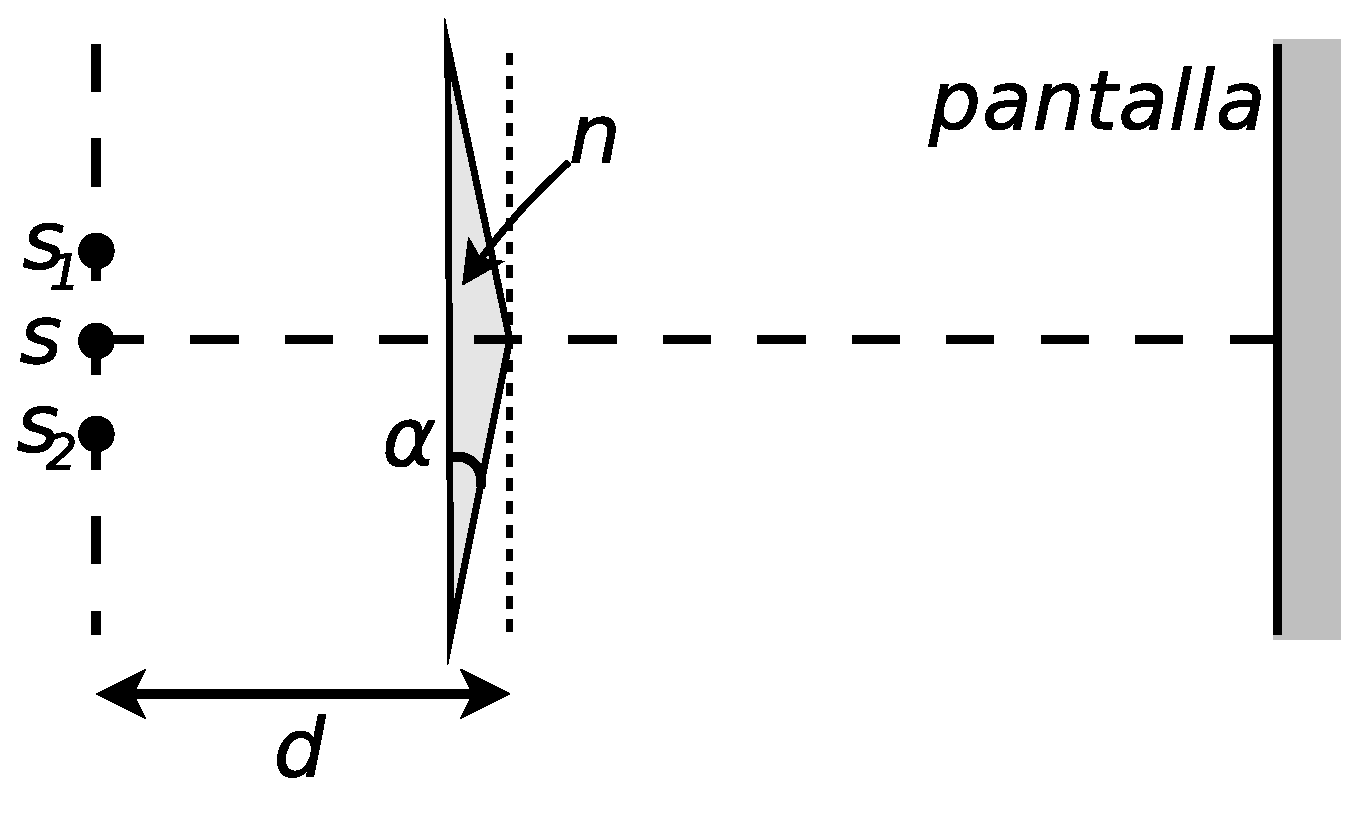
\includegraphics[width=\textwidth]{ej5-11}
\end{minipage}



\item Con vídrio Crown se construyó un biprisma de Fresnel con ángulo de \ang{1;;}.
Se ubica una pantalla a \SI{60}{\centi\metre} del biprisma y una fuente luminosa a \SI{15}{\centi\metre} de éste.
Calcular el ancho de las interfranjas observadas con luz roja (línea C de Fraunhofer) y luz azul (línea F de Fraunhofer).
Extraer las longitudes de onda y los índices de refracción de tablas.



\item Se observan franjas de interferencia con un biprisma de Fresnel con ángulo de \ang{1.5;;} e índice de refracción \num{1.5}.
Para esto se usa una fuente de luz de \SI{4000}{\angstrom} situada a \SI{5}{\centi\metre} del vértice, y una pantalla situada a \SI{1}{\metre} del biprisma.
Si, dejando todas las demás condiciones iguales, se cambia el biprisma por uno de ángulo \ang{3;;} e índice \num{1.6}; ¿en cuánto varió la interfranja?


\item En un experimento de interferencia con un biprisma de Fresnel, ¿qué parámetros se pueden modificar para que la interfranja aumente?


\item 
\begin{minipage}[t][3cm]{0.6\textwidth}
(*) Se tiene un dispositivo para producir interferencia consistente en una fuente puntual y monocromática $S$, que emite con longitud de onda $\lambda$, que se encuentra a una distancia $D_1$ de un biprisma compuesto por dos prismas delgados de distintos índices y ángulos: $n_1$, $\alpha_1$ ($y>0$) y $n_2$, $\alpha_2$ ($y<0$).
El dispositivo se muestra en la figura.
\end{minipage}
\begin{minipage}[c][2cm][t]{0.35\textwidth}
	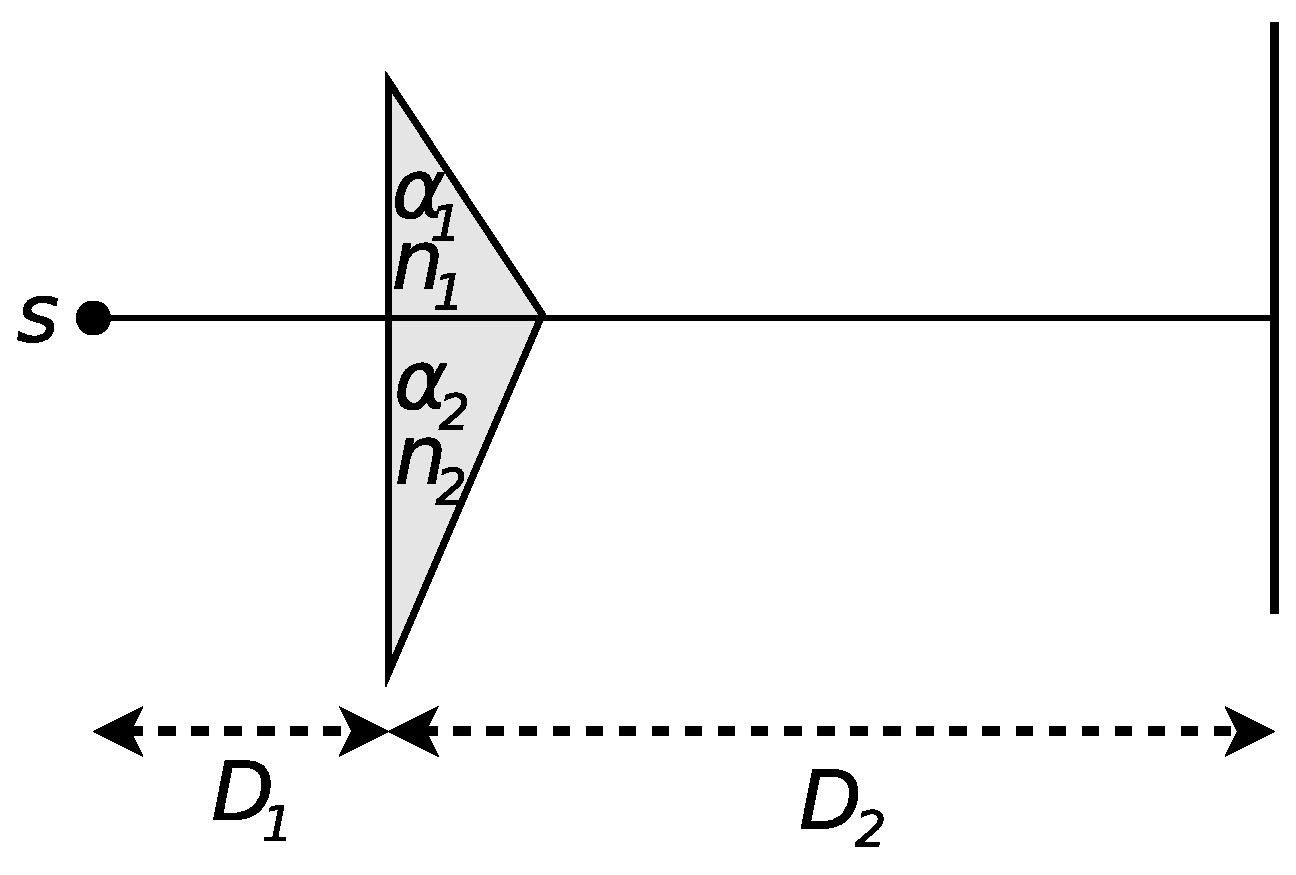
\includegraphics[width=\textwidth]{ej5-15}
\end{minipage}
\begin{enumerate}
	\item Hallar la ubicación de las imágenes $S_1$ y $S_2$ por la refracción en ambas zonas del biprisma, que observaría una persona ubicada a la derecha del mismo. 
	\item Marque en una figura la zona donde se produce la interferencia.
	\item Para un punto $P$ genérico sobre la pantalla, calcule el desfasaje $\delta$. Sugerencia: piense en los rayos que llegan a $P$ como provenientes de las imágenes halladas en a).
	\item Calcule la interfranja sobre la pantalla. 
	\item Halle la posición de los máximos sobre la pantalla.
	Si Ud. observara este fenómeno sin conocer los parámetros del dispositivo, ¿qué podría hacer para distinguir cuál es el orden con $m = 0$? 
	\item ¿Cómo debe ser la relación $\alpha_1/\alpha_2$ para que el máximo con $m = 0$ esté en la línea determinada por la fuente y el vértice del biprisma?
\end{enumerate}
